\documentclass[12pt]{article}
\usepackage{epsfig,amsmath,amssymb}
\usepackage{graphicx}
%\usepackage[]{fullpage}
%\usepackage{fancyhdr}
\usepackage{enumerate}
\usepackage{xfrac}
\usepackage{pgf}
\usepackage{pgfpages}
\usepackage{fix-cm}
\usepackage{hyperref}
\usepackage[margin=1in]{geometry}
\usepackage{caption}
\usepackage{dsfont}


\def\Z{\hbox{$\mathbb Z$}}
\def\Q{\hbox{$\mathbb Q$}}
\def\R{\hbox{$\mathbb R$}}
\def\F{\hbox{$\mathbb{F}$}}
\def\N{\hbox{$\mathbb N$}}
\def\C{\hbox{$\mathbb C$}}
\def\a{\hbox{$\alpha$}}
\def\b{\hbox{$\beta$}}
\def\g{\hbox{$\gamma$}}
\def\p{\hbox{$\rho$}}
\def\l{\hbox{$\lambda$}}
\newcommand{\li}[2][1]{\ensuremath{\displaystyle{\lim_{#1 \rightarrow #2}}}}
\newcommand{\su}[2][1]{\ensuremath{\displaystyle{\sum_{#1}^{#2}}}}
\renewcommand{\bf}{\mathbf}


% **** IF YOU WANT TO DEFINE ADDITIONAL MACROS FOR YOURSELF, PUT THEM HERE:

%\pagenumbering{gobble}

\renewcommand{\thetable}{\arabic{table}}

\begin{document}
\section*{Phase 1}
\subsection*{Iteration 1}

\renewcommand{\arraystretch}{1.5}
$\begin{array}{c|rrrrrrrrrrrr|r|}
\cline{2-13}
& w_1 & w_2 & w_3 & w_4 & w_5 & w_6 & z_1 & z_2 & z_3 & z_4 & z_5 & z_6 \\
\cline{2-14}
w_1 & 1 & 0 & 0 & 0 & 0 & 0 & 0 & 0 & 0 & 1 & 0 & 0 & 3 \\
w_2 & 0 & 1 & 0 & 0 & 0 & 0 & 0 & 0 & 0 & 0 & 1 & 0 & 2 \\
w_3 & 0 & 0 & 1 & 0 & 0 & 0 & 0 & 0 & 0 & 0 & -1 & 0 & 3 x_{12} - 2 \\
w_4 & 0 & 0 & 0 & 1 & 0 & 0 & -1 & 0 & 0 & - 2 x_{11} - 1 & x_{11} + 2 & - 2 x_{11} - 1 & x_{11} + 2 x_{12} - 1 \\
w_5 & 0 & 0 & 0 & 0 & 1 & 0 & 0 & -1 & 1 & x_{11} + 2 & x_{11} - 8 & 4 x_{11} + 1 & - 2 x_{11} + 2 x_{12} - 1 \\
w_6 & 0 & 0 & 0 & 0 & 0 & 1 & 0 & 0 & 0 & - 2 x_{11} - 1 & 4 x_{11} + 1 & - 2 x_{11} - 2 & 1 - x_{11} \\
\cline{2-14}
\end{array}$

\begin{center}
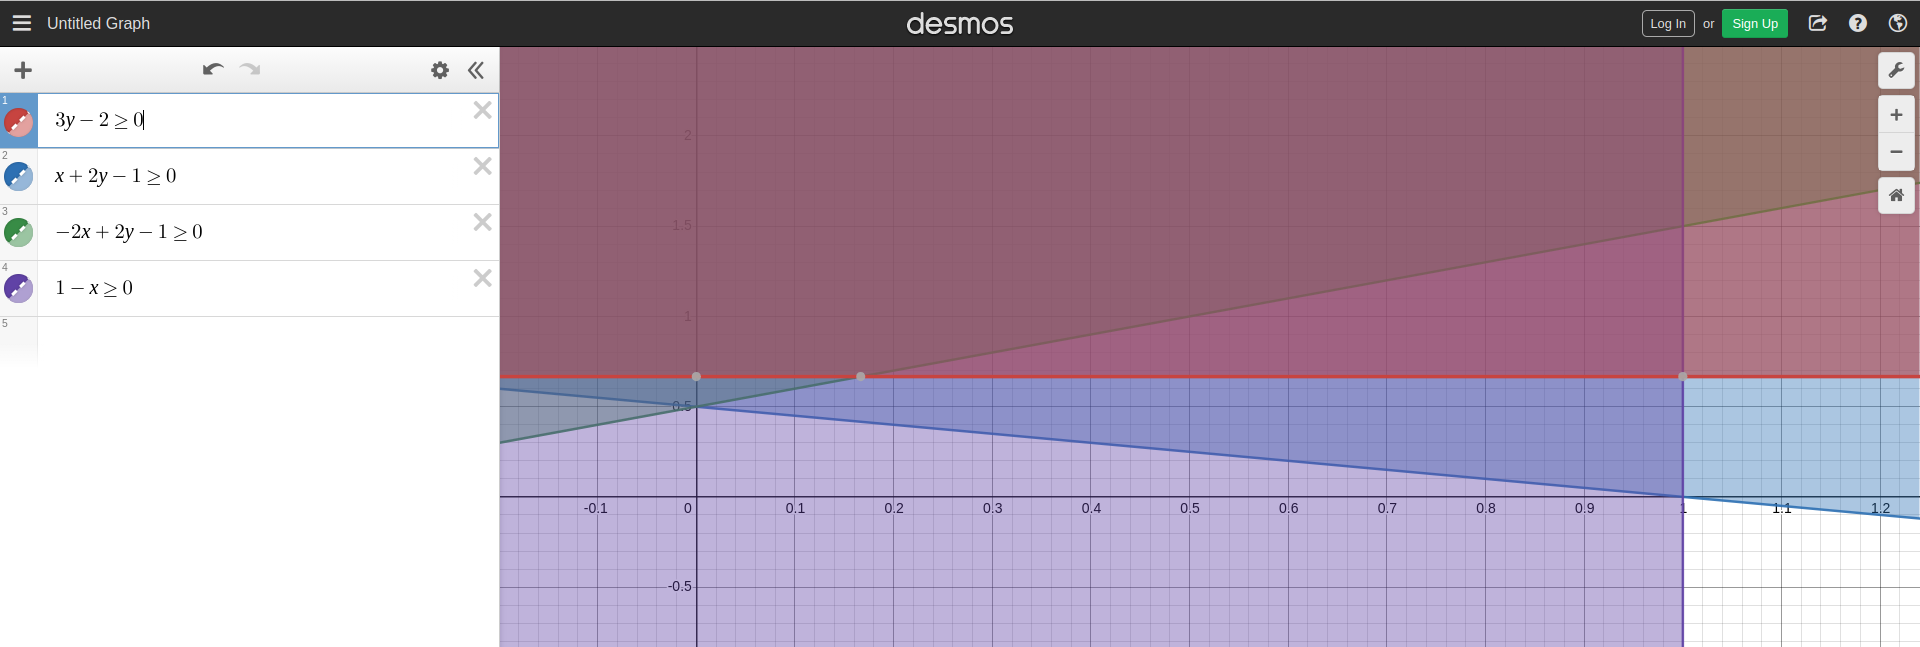
\includegraphics[scale=.3]{Phase1_iteration1_visual}
\end{center}

Perform exchange pivot for $w_3 \rightarrow z_3$ and $w_5 \rightarrow z_5$.


\subsection*{Iteration 2}
{\footnotesize
$\begin{array}{c|rrrrrrrrrrrr|r|}
\cline{2-13}
& w_1 & w_2 & w_3 & w_4 & w_5 & w_6 & z_1 & z_2 & z_3 & z_4 & z_5 & z_6 \\
\cline{2-14}
w_1 & 1 & 0 & 0 & 0 & 0 & 0 & 0 & 0 & 0 & 1 & 0 & 0 & 3 \\
w_2 & 0 & 1 & 1 & 0 & 0 & 0 & 0 & 0 & 0 & 0 & 0 & 0 & 3 x_{12} \\
z_3 & 0 & 0 & x_{11} - 8 & 0 & 1 & 0 & 0 & -1 & 1 & x_{11} + 2 & 0 & 4 x_{11} + 1 & 3 x_{11} x_{12} - 4 x_{11} - 22 x_{12} + 15 \\
w_4 & 0 & 0 & x_{11} + 2 & 1 & 0 & 0 & -1 & 0 & 0 & - 2 x_{11} - 1 & 0 & - 2 x_{11} - 1 & 3 x_{11} x_{12} - x_{11} + 8 x_{12} - 5 \\
z_5 & 0 & 0 & -1 & 0 & 0 & 0 & 0 & 0 & 0 & 0 & 1 & 0 & 2 - 3 x_{12} \\
w_6 & 0 & 0 & 4 x_{11} + 1 & 0 & 0 & 1 & 0 & 0 & 0 & - 2 x_{11} - 1 & 0 & - 2 x_{11} - 2 & - x_{11} + \left(4 x_{11} + 1\right) \left(3 x_{12} - 2\right) + 1 \\
\cline{2-14}
\end{array}$
}

\begin{center}
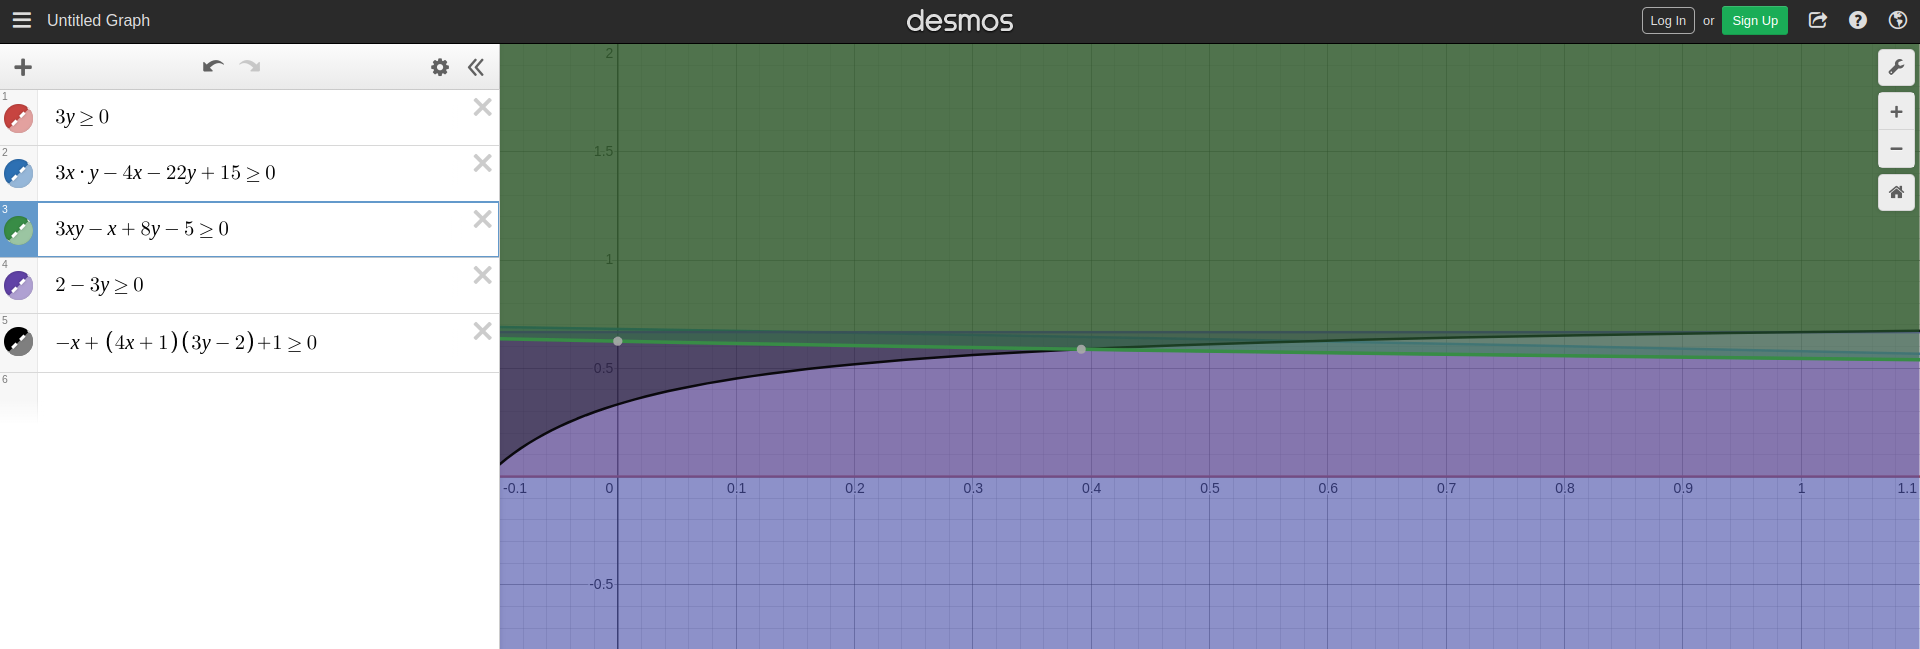
\includegraphics[scale=.3]{Phase1_iteration2_visual}
\end{center}

Perform diagonal pivot for $w_4 \rightarrow z_4$.


\subsection*{Iteration 3}
{\scriptsize
$\begin{array}{c|rrrrrrrrrrrr|r|}
\cline{2-13}
& w_1 & w_2 & w_3 & w_4 & w_5 & w_6 & z_1 & z_2 & z_3 & z_4 & z_5 & z_6 \\
\cline{2-14}
w_1 & 1 & 0 & \frac{x_{11} + 2}{2 x_{11} + 1} & \frac{1}{2 x_{11} + 1} & 0 & 0 & - \frac{1}{2 x_{11} + 1} & 0 & 0 & 0 & 0 & -1 & \frac{3 x_{11} x_{12} + 5 x_{11} + 8 x_{12} - 2}{2 x_{11} + 1} \\
w_2 & 0 & 1 & 1 & 0 & 0 & 0 & 0 & 0 & 0 & 0 & 0 & 0 & 3 x_{12} \\
z_3 & 0 & 0 & \frac{3 x_{11}^{2} - 11 x_{11} - 4}{2 x_{11} + 1} & \frac{x_{11} + 2}{2 x_{11} + 1} & 1 & 0 & - \frac{x_{11} + 2}{2 x_{11} + 1} & -1 & 1 & 0 & 0 & 3 x_{11} - 1 & \frac{9 x_{11}^{2} x_{12} - 9 x_{11}^{2} - 27 x_{11} x_{12} + 19 x_{11} - 6 x_{12} + 5}{2 x_{11} + 1} \\
z_4 & 0 & 0 & - \frac{x_{11} + 2}{2 x_{11} + 1} & - \frac{1}{2 x_{11} + 1} & 0 & 0 & \frac{1}{2 x_{11} + 1} & 0 & 0 & 1 & 0 & 1 & \frac{- 3 x_{11} x_{12} + x_{11} - 8 x_{12} + 5}{2 x_{11} + 1} \\
z_5 & 0 & 0 & -1 & 0 & 0 & 0 & 0 & 0 & 0 & 0 & 1 & 0 & 2 - 3 x_{12} \\
w_6 & 0 & 0 & 3 x_{11} - 1 & -1 & 0 & 1 & 1 & 0 & 0 & 0 & 0 & -1 & 9 x_{11} x_{12} - 8 x_{11} - 5 x_{12} + 4 \\
\cline{2-14}
\end{array}$
}

\begin{center}
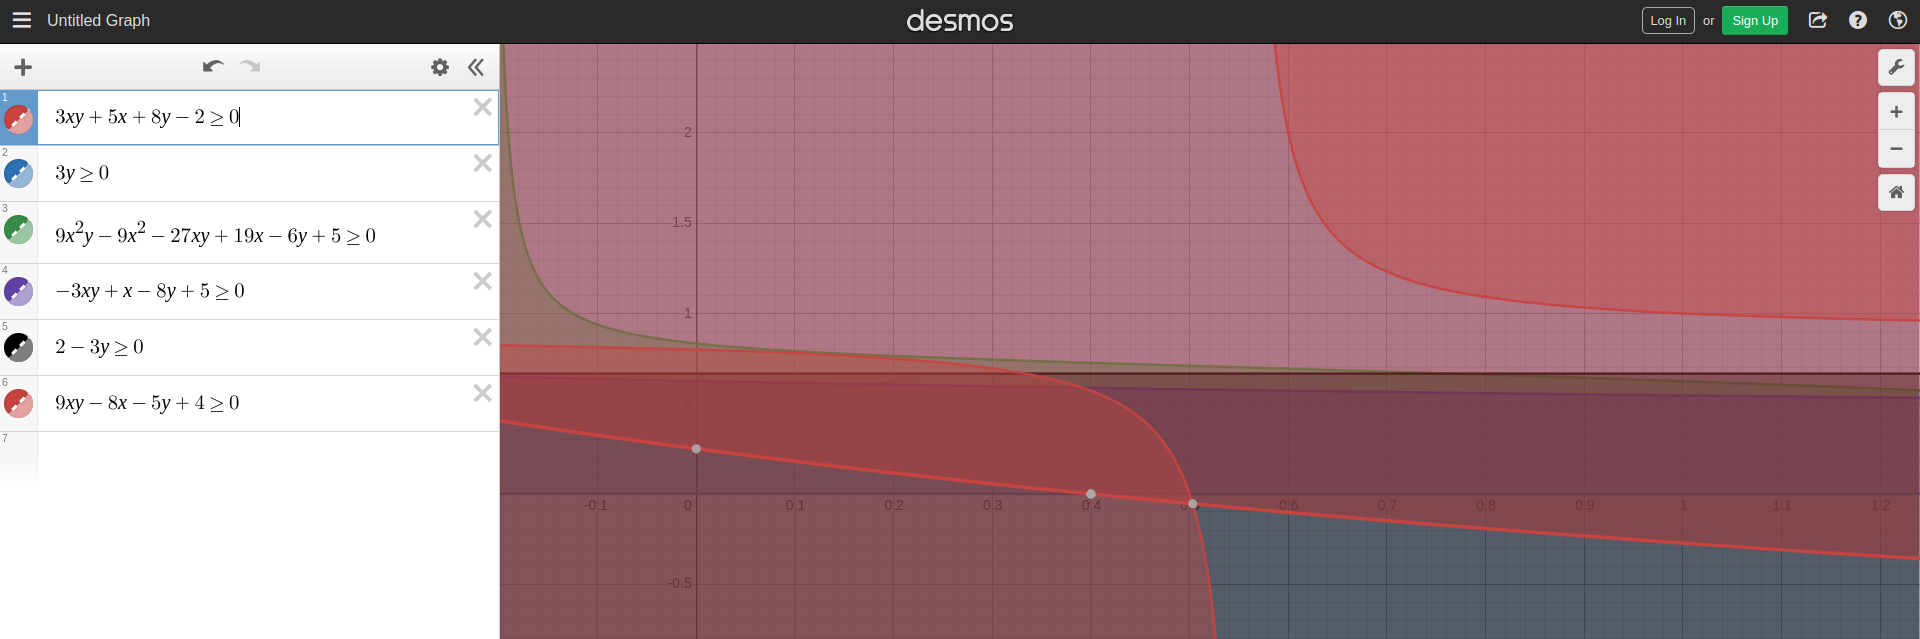
\includegraphics[scale=.3]{Phase1_iteration3_visual}
\end{center}

This region is valid for $ 0.4 \leq x_{11} \leq 0.5 $ with $x_{12} = 0$, so we move to phase 2.

\section*{Phase 2}
\subsection*{Iteration 1}

$\begin{array}{c|rrrrrrrrrrrr|r|}
\cline{2-13}
& w_1 & w_2 & w_3 & w_4 & w_5 & w_6 & z_1 & z_2 & z_3 & z_4 & z_5 & z_6 \\
\cline{2-14}
w_1 & 1 & 0 & \frac{x_{11} + 2}{2 x_{11} + 1} & \frac{1}{2 x_{11} + 1} & 0 & 0 & - \frac{1}{2 x_{11} + 1} & 0 & 0 & 0 & 0 & -1 & \frac{5 x_{11} - 2}{2 x_{11} +1} \\
w_2 & 0 & 1 & 1 & 0 & 0 & 0 & 0 & 0 & 0 & 0 & 0 & 0 & 0 \\
z_3 & 0 & 0 & \frac{3 x_{11}^{2} - 11 x_{11} - 4}{2 x_{11} + 1} & \frac{x_{11} + 2}{2 x_{11} + 1} & 1 & 0 & - \frac{x_{11} + 2}{2 x_{11} + 1} & -1 & 1 & 0 & 0 & 3 x_{11} - 1 & \frac{- 9 x_{11}^{2} + 19 x_{11} + 5}{2 x_{11} + 1} \\
z_4 & 0 & 0 & - \frac{x_{11} + 2}{2 x_{11} + 1} & - \frac{1}{2 x_{11} + 1} & 0 & 0 & \frac{1}{2 x_{11} + 1} & 0 & 0 & 1 & 0 & 1 & \frac{x_{11} + 5}{2 x_{11} + 1} \\
z_5 & 0 & 0 & -1 & 0 & 0 & 0 & 0 & 0 & 0 & 0 & 1 & 0 & 2 \\
w_6 & 0 & 0 & 3 x_{11} - 1 & -1 & 0 & 1 & 1 & 0 & 0 & 0 & 0 & -1 & 4 - 8 x_{11} \\
\cline{2-14}
\end{array}$

\begin{center}
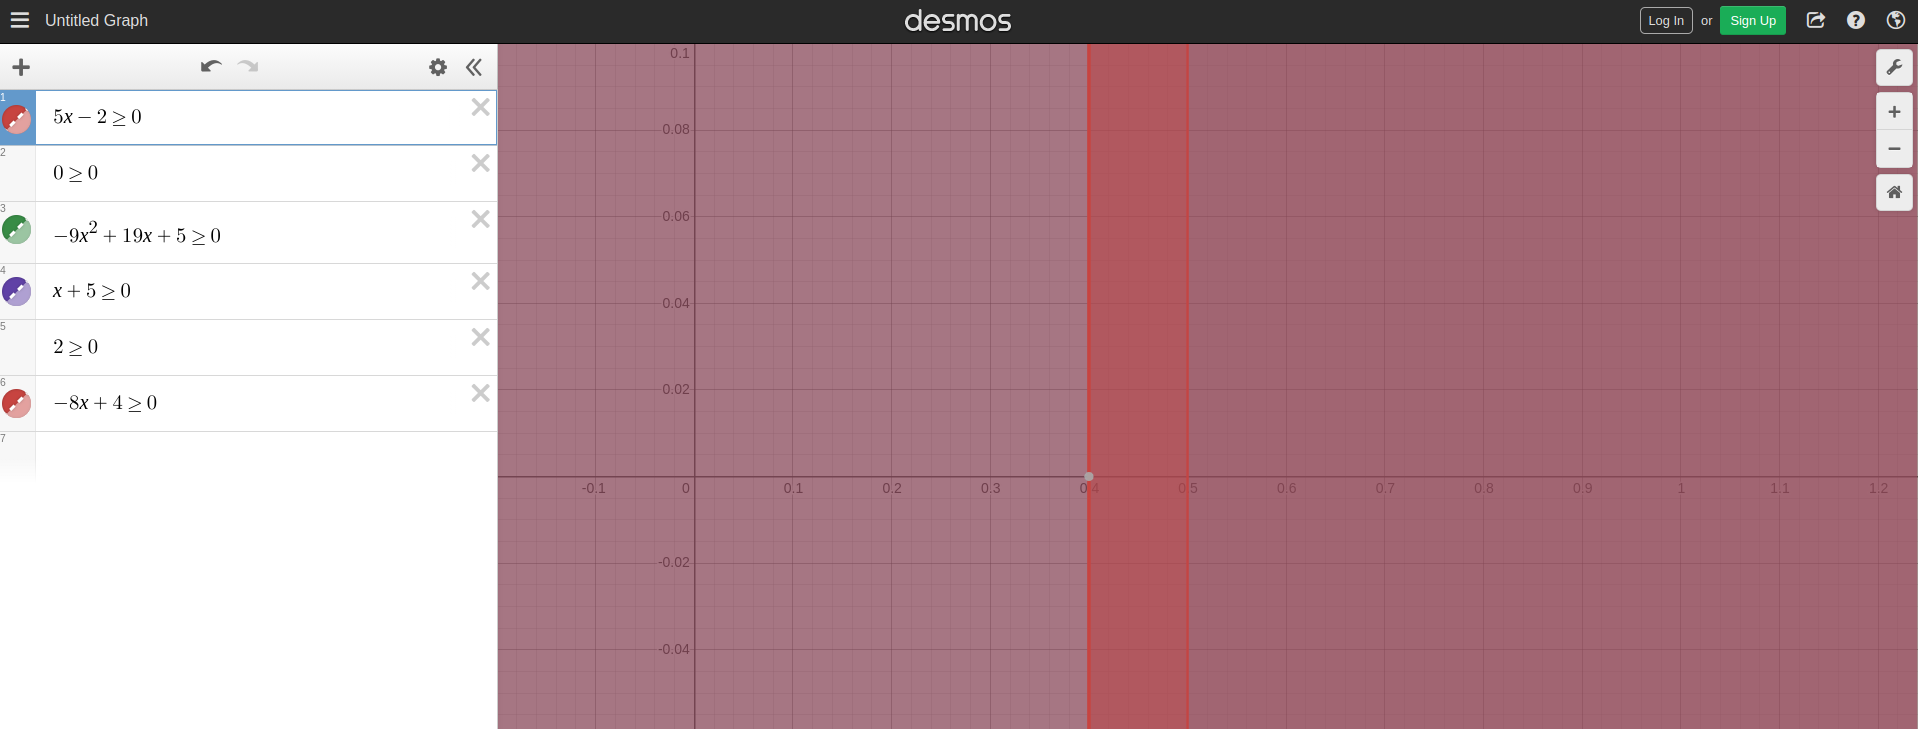
\includegraphics[scale=.3]{Phase2_iteration1_visual}
\end{center}

Perform diagonal pivot for $w_1 \rightarrow z_1$.

\subsection*{Iteration 2}

$\begin{array}{c|rrrrrrrrrrrr|r|}
\cline{2-13}
& w_1 & w_2 & w_3 & w_4 & w_5 & w_6 & z_1 & z_2 & z_3 & z_4 & z_5 & z_6 \\
\cline{2-14}
z_1 & - 2 x_{11} - 1 & 0 & - x_{11} - 2 & -1 & 0 & 0 & 1 & 0 & 0 & 0 & 0 & 2 x_{11} + 1 & 2 - 5 x_{11} \\
w_2 & 0 & 1 & 1 & 0 & 0 & 0 & 0 & 0 & 0 & 0 & 0 & 0 & 0 \\
z_3 & - x_{11} - 2 & 0 & x_{11} - 8 & 0 & 1 & 0 & 0 & -1 & 1 & 0 & 0 & 4 x_{11} + 1 & 9 - 7 x_{11} \\
z_4 & 1 & 0 & 0 & 0 & 0 & 0 & 0 & 0 & 0 & 1 & 0 & 0 & 3 \\
z_5 & 0 & 0 & -1 & 0 & 0 & 0 & 0 & 0 & 0 & 0 & 1 & 0 & 2 \\
w_6 & 2 x_{11} + 1 & 0 & 4 x_{11} + 1 & 0 & 0 & 1 & 0 & 0 & 0 & 0 & 0 & - 2 x_{11} - 2 & 2 - 3 x_{11} \\
\cline{2-14}
\end{array}$

\begin{center}
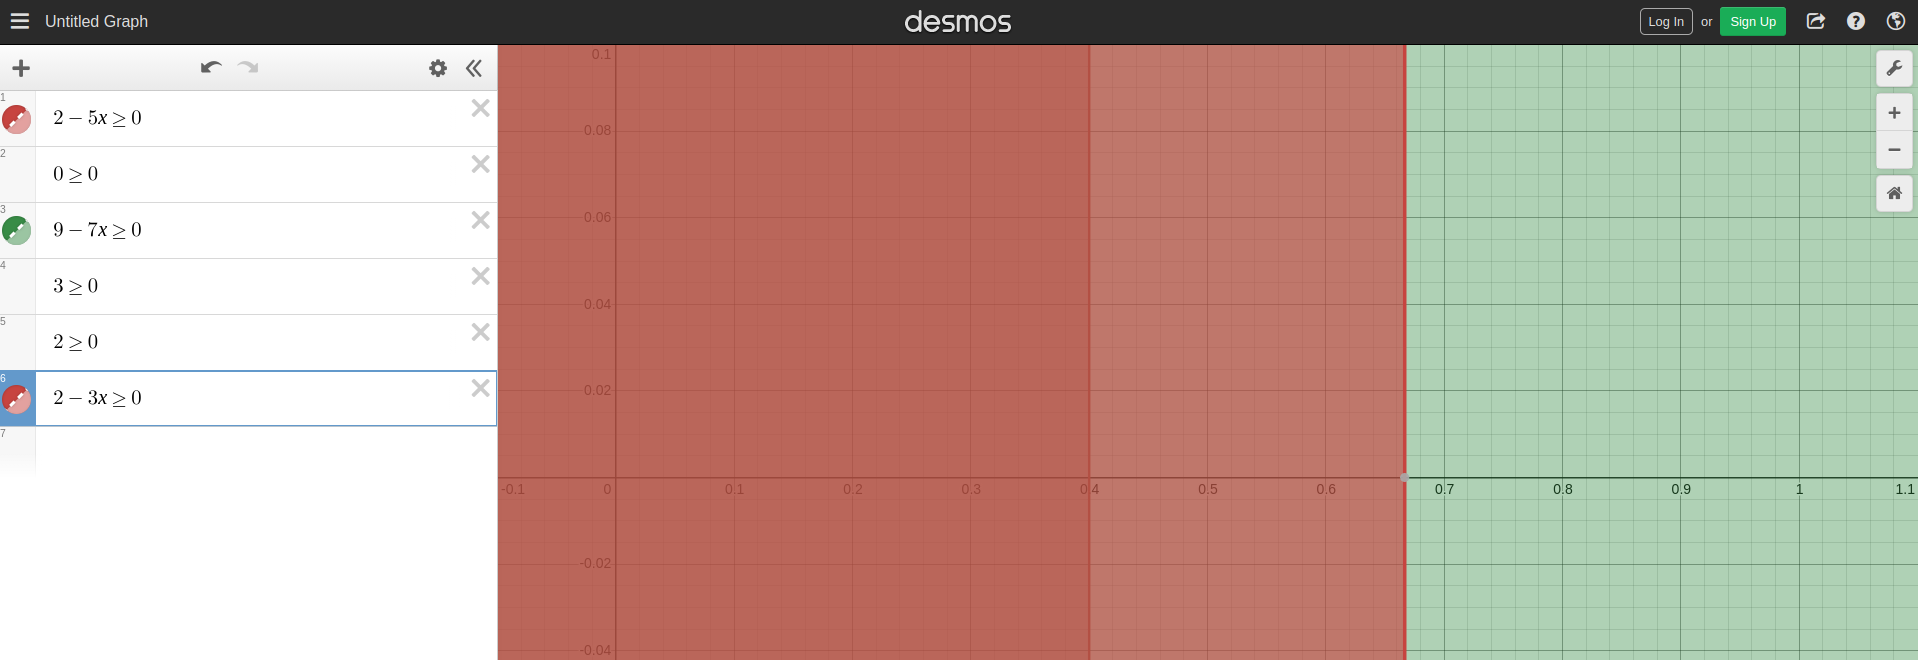
\includegraphics[scale=.3]{Phase2_iteration2_visual}
\end{center}

Solution is valid for $0 \leq x_{11} \leq 0.4$, so for iteration 3, return to tableau of iteration 1 and perform diagonal pivot for $w_6 \rightarrow z_6$.


\subsection*{Iteration 3}

$\begin{array}{c|rrrrrrrrrrrr|r|}
\cline{2-13}
& w_1 & w_2 & w_3 & w_4 & w_5 & w_6 & z_1 & z_2 & z_3 & z_4 & z_5 & z_6 \\
\cline{2-14}
z_1 & 1 & 0 & \frac{3 - 6 x_{11}^{2}}{2 x_{11} + 1} & \frac{2 \left(x_{11} + 1\right)}{2 x_{11} + 1} & 0 & -1 & - \frac{2 x_{11} + 2}{2 x_{11} + 1} & 0 & 0 & 0& 0 & 0 & \frac{16 x_{11}^{2} + 5 x_{11} - 6}{2 x_{11} + 1} \\
w_2 & 0 & 1 & 1 & 0 & 0 & 0 & 0 & 0 & 0 & 0 & 0 & 0 & 0 \\
z_3 & 0 & 0 & \frac{3 \left(6 x_{11}^{3} - 5 x_{11} - 1\right)}{2 x_{11} + 1} & \frac{3 - 6 x_{11}^{2}}{2 x_{11} + 1} & 1 & 3 x_{11} - 1 & \frac{3 \left(2 x_{11}^{2} - 1\right)}{2 x_{11} + 1} & -1 & 1 & 0 & 0 & 0 & \frac{- 48 x_{11}^{3} + 7 x_{11}^{2} + 31 x_{11} + 1}{2 x_{11} + 1} \\
z_4 & 0 & 0 & \frac{3 \left(2 x_{11}^{2} - 1\right)}{2 x_{11} + 1} & - \frac{2 x_{11} + 2}{2 x_{11} + 1} & 0 & 1 & \frac{2 \left(x_{11} + 1\right)}{2 x_{11} + 1} & 0 & 0 & 1 & 0 & 0 & \frac{- 16 x_{11}^{2} + x_{11} + 9}{2 x_{11} + 1} \\
z_5 & 0 & 0 & -1 & 0 & 0 & 0 & 0 & 0 & 0 & 0 & 1 & 0 & 2 \\
z_6 & 0 & 0 & 1 - 3 x_{11} & 1 & 0 & -1 & -1 & 0 & 0 & 0 & 0 & 1 & 8 x_{11} - 4 \\
\cline{2-14}
\end{array}$

\begin{center}
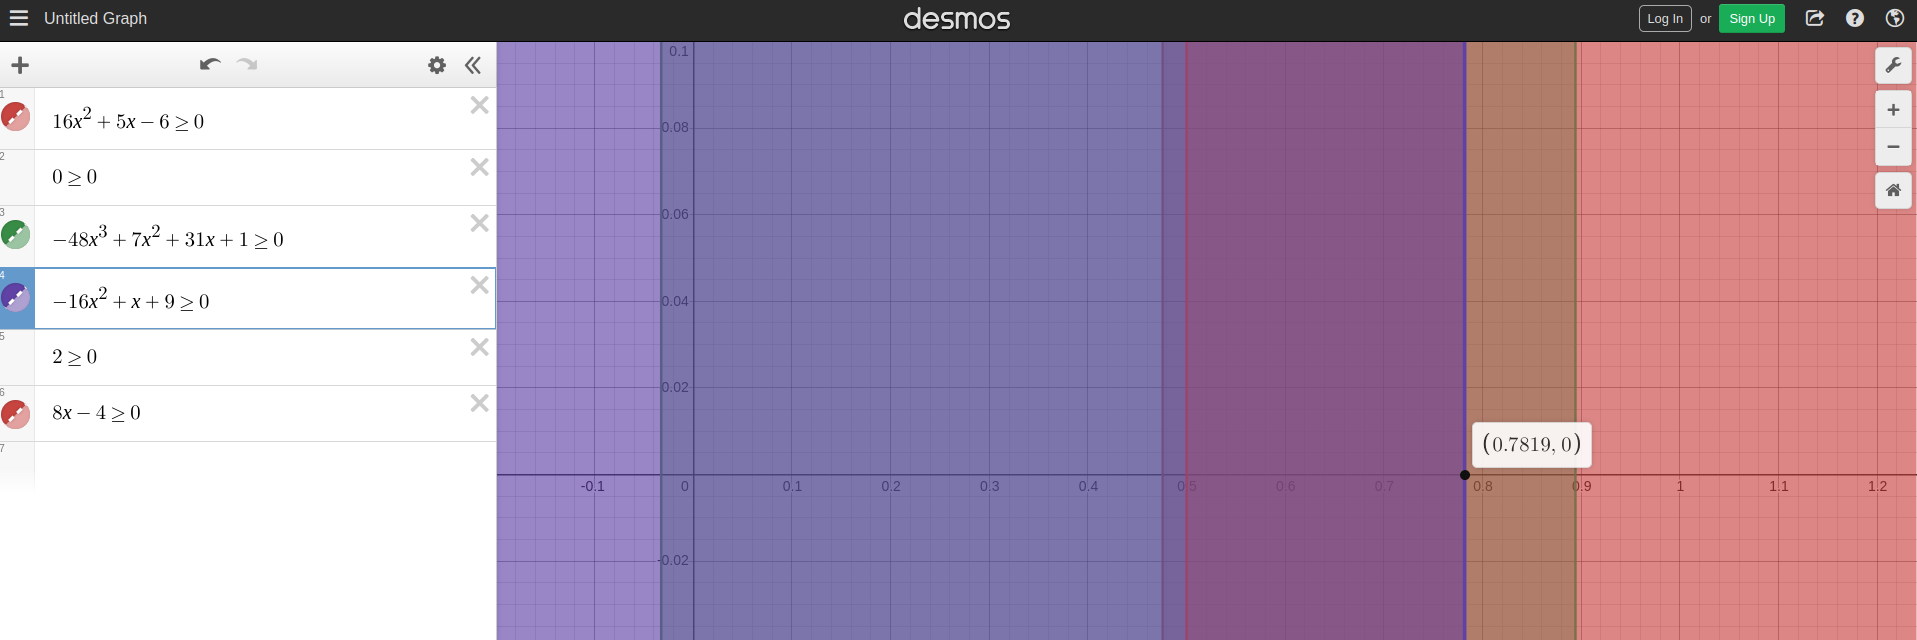
\includegraphics[scale=.3]{Phase2_iteration3_visual}
\end{center}

Perform diagonal pivot for $z_4 \rightarrow w_4$.

\subsection*{Iteration 4}

$\begin{array}{c|rrrrrrrrrrrr|r|}
\cline{2-13}
& w_1 & w_2 & w_3 & w_4 & w_5 & w_6 & z_1 & z_2 & z_3 & z_4 & z_5 & z_6 \\
\cline{2-14}
z_1 & 1 & 0 & 0 & 0 & 0 & 0 & 0 & 0 & 0 & 1 & 0 & 0 & 3 \\
w_2 & 0 & 1 & 1 & 0 & 0 & 0 & 0 & 0 & 0 & 0 & 0 & 0 & 0 \\
z_3 & 0 & 0 & \frac{3 \left(6 x_{11}^{2} - 2 x_{11} - 5\right)}{2 \left(x_{11} + 1\right)} & 0 & 1 & \frac{4 x_{11} + 1}{2 \left(x_{11} + 1\right)} & 0 & -1 & 1 & \frac{3 \left(1 - 2 x_{11}^{2}\right)}{2 \left(x_{11} + 1\right)} & 0 & 0 & \frac{- 44 x_{11}^{2} + 9 x_{11} + 29}{2 x_{11} + 2} \\
w_4 & 0 & 0 & \frac{3 \left(1 - 2 x_{11}^{2}\right)}{2 \left(x_{11} + 1\right)} & 1 & 0 & - \frac{x_{11} + \frac{1}{2}}{x_{11} + 1} & -1 & 0 & 0 & - \frac{x_{11} + \frac{1}{2}}{x_{11} + 1} & 0 & 0 & \frac{16 x_{11}^{2} - x_{11} - 9}{2 \left(x_{11} + 1\right)} \\
z_5 & 0 & 0 & -1 & 0 & 0 & 0 & 0 & 0 & 0 & 0 & 1 & 0 & 2 \\
z_6 & 0 & 0 & - \frac{4 x_{11} + 1}{2 x_{11} + 2} & 0 & 0 & - \frac{1}{2 x_{11} + 2} & 0 & 0 & 0 & \frac{x_{11} + \frac{1}{2}}{x_{11} + 1} & 0 & 1 & \frac{9 x_{11} + 1}{2 \left(x_{11} + 1\right)} \\
\cline{2-14}
\end{array}$

\begin{center}
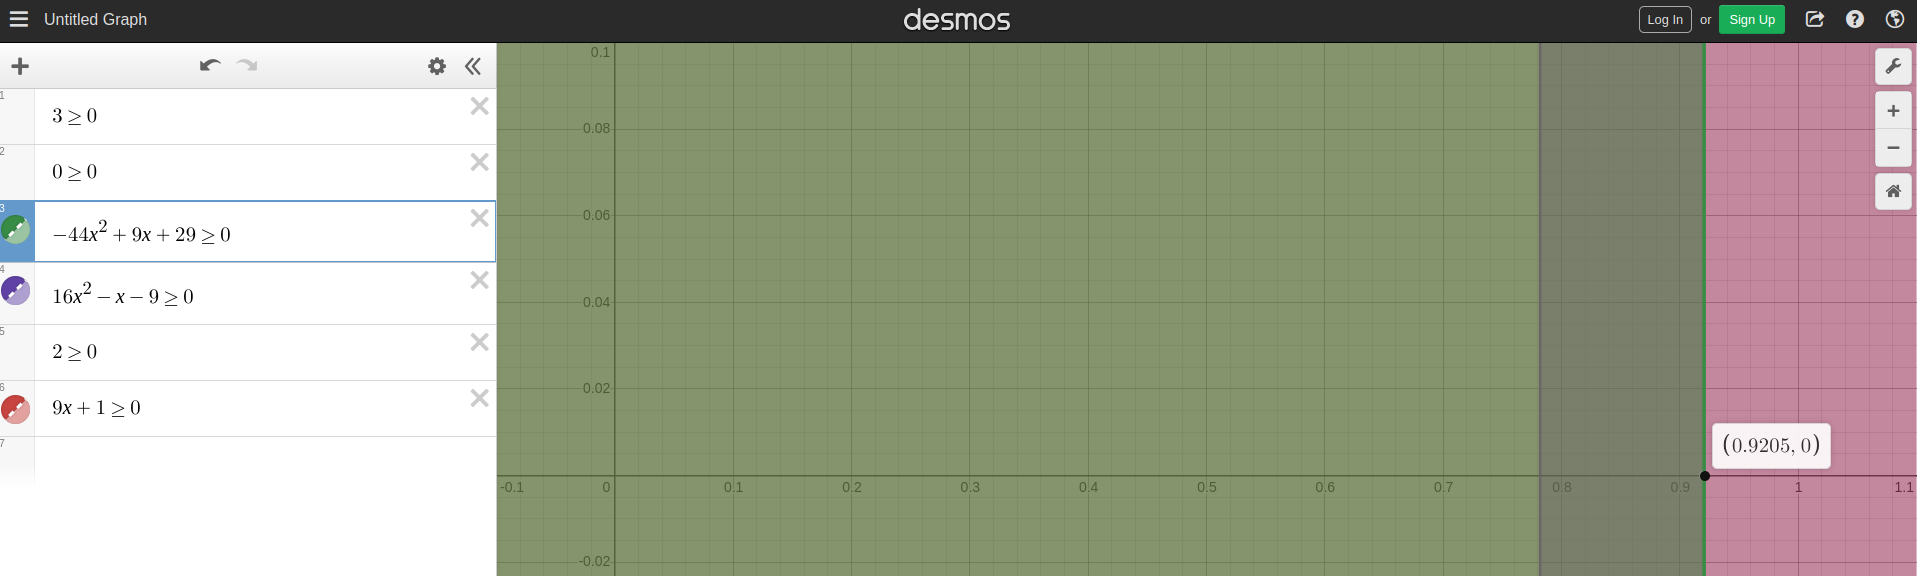
\includegraphics[scale=.3]{Phase2_iteration4_visual}
\end{center}

Perform diagonal pivot for $z_3 \rightarrow w_3$.


\subsection*{Iteration 5}

{\footnotesize
$\begin{array}{c|rrrrrr|r|}
\cline{2-7}
& w_1 & w_2 & w_3 & w_4 & w_5 & w_6 \\
\cline{2-7}
z_1 & 1 & 0 & 0 & 0 & 0 & 0 \\
w_2 & 0 & 1 & 0 & 0 & \frac{2 \left(x_{11} + 1\right)}{3 \left(- 6 x_{11}^{2} + 2 x_{11} + 5\right)} & \frac{4 x_{11} + 1}{3 \left(- 6 x_{11}^{2} + 2 x_{11} + 5\right)} \\
w_3 & 0 & 0 & 1 & 0 & \frac{2 \left(x_{11} + 1\right)}{3 \left(6 x_{11}^{2} - 2 x_{11} - 5\right)} & \frac{4 x_{11} + 1}{3 \left(6 x_{11}^{2} - 2 x_{11} - 5\right)} \\
w_4 & 0 & 0 & 0 & 1 & \frac{1 - 2 x_{11}^{2}}{- 6 x_{11}^{2} + 2 x_{11} + 5} & \frac{- 2 x_{11}^{2} + 2 x_{11} + 2}{6 x_{11}^{2} - 2 x_{11} - 5} \\
z_5 & 0 & 0 & 0 & 0 & \frac{2 \left(x_{11} + 1\right)}{3 \left(6 x_{11}^{2} - 2 x_{11} - 5\right)} & \frac{4 x_{11} + 1}{3 \left(6 x_{11}^{2} - 2 x_{11} - 5\right)} \\
z_6 & 0 & 0 & 0 & 0 & \frac{4 x_{11} + 1}{3 \left(6 x_{11}^{2} - 2 x_{11} - 5\right)} & \frac{x_{11} - 8}{- 18 x_{11}^{2} + 6 x_{11} + 15} \\
\cline{2-7}
& z_1 & z_2 & z_3 & z_4 & z_5 & z_6 \\
\cline{2-8}
z_1 & 0 & 0 & 0 & 1 & 0 & 0 & 3 \\
w_2 & 0 & \frac{2 \left(x_{11} + 1\right)}{3 \left(6 x_{11}^{2} - 2 x_{11} - 5\right)} & \frac{2 \left(x_{11} + 1\right)}{3 \left(- 6 x_{11}^{2} + 2 x_{11} + 5\right)} & \frac{1 - 2 x_{11}^{2}}{- 6 x_{11}^{2} + 2 x_{11} + 5} & 0 & 0 & \frac{- 44 x_{11}^{2} + 9 x_{11} + 29}{3 \left(- 6 x_{11}^{2} + 2 x_{11} + 5\right)}\\
w_3 & 0 & \frac{2 \left(x_{11} + 1\right)}{3 \left(- 6 x_{11}^{2} + 2 x_{11} + 5\right)} & \frac{2 \left(x_{11} + 1\right)}{3 \left(6 x_{11}^{2} - 2 x_{11} - 5\right)} & \frac{2 x_{11}^{2} - 1}{- 6 x_{11}^{2} + 2 x_{11} + 5} & 0 & 0 & - \frac{- 44 x_{11}^{2} + 9 x_{11} + 29}{- 18 x_{11}^{2} + 6 x_{11} + 15} \\
w_4 & -1 & \frac{2 x_{11}^{2} - 1}{- 6 x_{11}^{2} + 2 x_{11} + 5} & \frac{1 - 2 x_{11}^{2}}{- 6 x_{11}^{2} + 2 x_{11} + 5} & \frac{- 6 x_{11}^{3} + 5 x_{11} + 1}{6 x_{11}^{2} - 2 x_{11} - 5} & 0 & 0 & \frac{4 x_{11}^{3} - 14 x_{11}^{2} - x_{11} + 8}{6 x_{11}^{2} - 2 x_{11} - 5} \\
z_5 & 0 & \frac{2 \left(x_{11} + 1\right)}{3 \left(- 6 x_{11}^{2} + 2 x_{11} + 5\right)} & \frac{2 \left(x_{11} + 1\right)}{3 \left(6 x_{11}^{2} - 2 x_{11} - 5\right)} & \frac{2 x_{11}^{2} - 1}{- 6 x_{11}^{2} + 2 x_{11} + 5} & 1 & 0 & \frac{8 x_{11}^{2} + 3 x_{11} + 1}{3 \left(- 6 x_{11}^{2} + 2 x_{11} + 5\right)} \\
z_6 & 0 & \frac{4 x_{11} + 1}{3 \left(- 6 x_{11}^{2} + 2 x_{11} + 5\right)} & \frac{4 x_{11} + 1}{3 \left(6 x_{11}^{2} - 2 x_{11} - 5\right)} & \frac{2 \left(x_{11}^{2} - x_{11} - 1\right)}{6 x_{11}^{2} - 2 x_{11} - 5} & 0 & 1 & \frac{7 x_{11}^{2} + 15 x_{11} - 7}{- 18 x_{11}^{2} + 6 x_{11} + 15} \\
\cline{2-8}
\end{array}$
}

\begin{center}
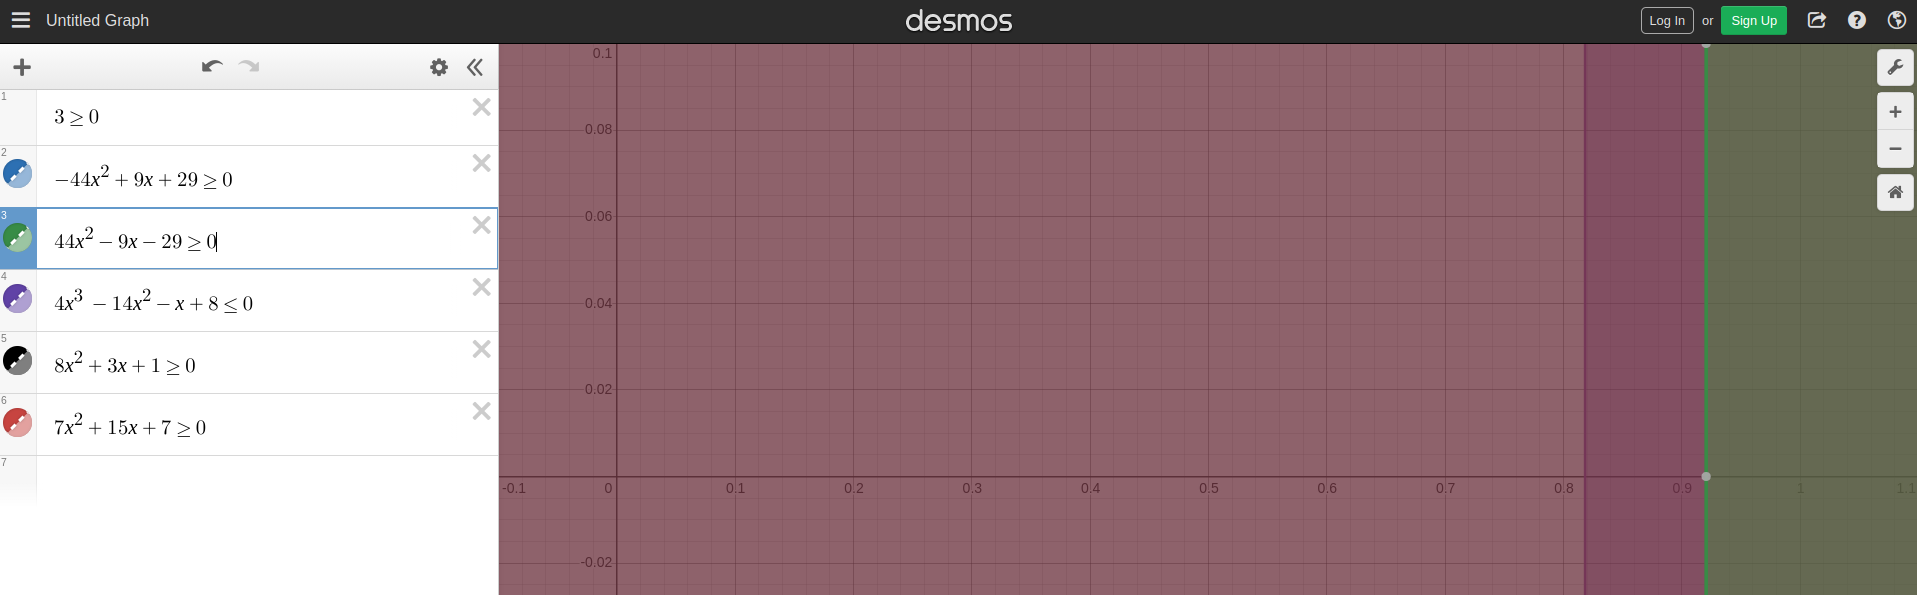
\includegraphics[scale=.3]{Phase2_iteration5_visual}
\end{center}

Boundaries associated with $w_2$ and $w_3$ overlap and create 0-dimensional invariancy region. Perform diagonal pivot for $w_2 \rightarrow z_2$.

\subsection*{Iteration 6}

\renewcommand{\arraystretch}{1.5}
$\begin{array}{c|rrrrrrrrrrrr|r|}
\cline{2-13}
& w_1 & w_2 & w_3 & w_4 & w_5 & w_6 & z_1 & z_2 & z_3 & z_4 & z_5 & z_6 \\
\cline{2-14}
z_1 & 1 & 0 & 0 & 0 & 0 & 0 & 0 & 0 & 0 & 1 & 0 & 0 & 3 \\
z_2 & 0 & \frac{3 \left(6 x_{11}^{2} - 2 x_{11} - 5\right)}{2 \left(x_{11} + 1\right)} & 0 & 0 & -1 & - \frac{4 x_{11} + 1}{2 x_{11} + 2} & 0 & 1 & -1 & \frac{3 \left(2 x_{11}^{2} - 1\right)}{2 \left(x_{11} + 1\right)} & 0 & 0 & \frac{44 x_{11}^{2} - 9 x_{11} - 29}{2 \left(x_{11} + 1\right)} \\
w_3 & 0 & 1 & 1 & 0 & 0 & 0 & 0 & 0 & 0 & 0 & 0 & 0 & 0 \\
w_4 & 0 & \frac{3 \left(2 x_{11}^{2} - 1\right)}{2 \left(x_{11} + 1\right)} & 0 & 1 & 0 & - \frac{x_{11} + \frac{1}{2}}{x_{11} + 1} & -1 & 0 & 0 & - \frac{x_{11} + \frac{1}{2}}{x_{11} + 1} & 0 & 0 & \frac{16 x_{11}^{2} - x_{11} - 9}{2 \left(x_{11} + 1\right)} \\
z_5 & 0 & 1 & 0 & 0 & 0 & 0 & 0 & 0 & 0 & 0 & 1 & 0 & 2 \\
z_6 & 0 & \frac{4 x_{11} + 1}{2 \left(x_{11} + 1\right)} & 0 & 0 & 0 & - \frac{1}{2 x_{11} + 2} & 0 & 0 & 0 & \frac{x_{11} + \frac{1}{2}}{x_{11} + 1} & 0 & 1 &\frac{9 x_{11} + 1}{2 \left(x_{11} + 1\right)} \\
\cline{2-14}
\end{array}$

\begin{center}
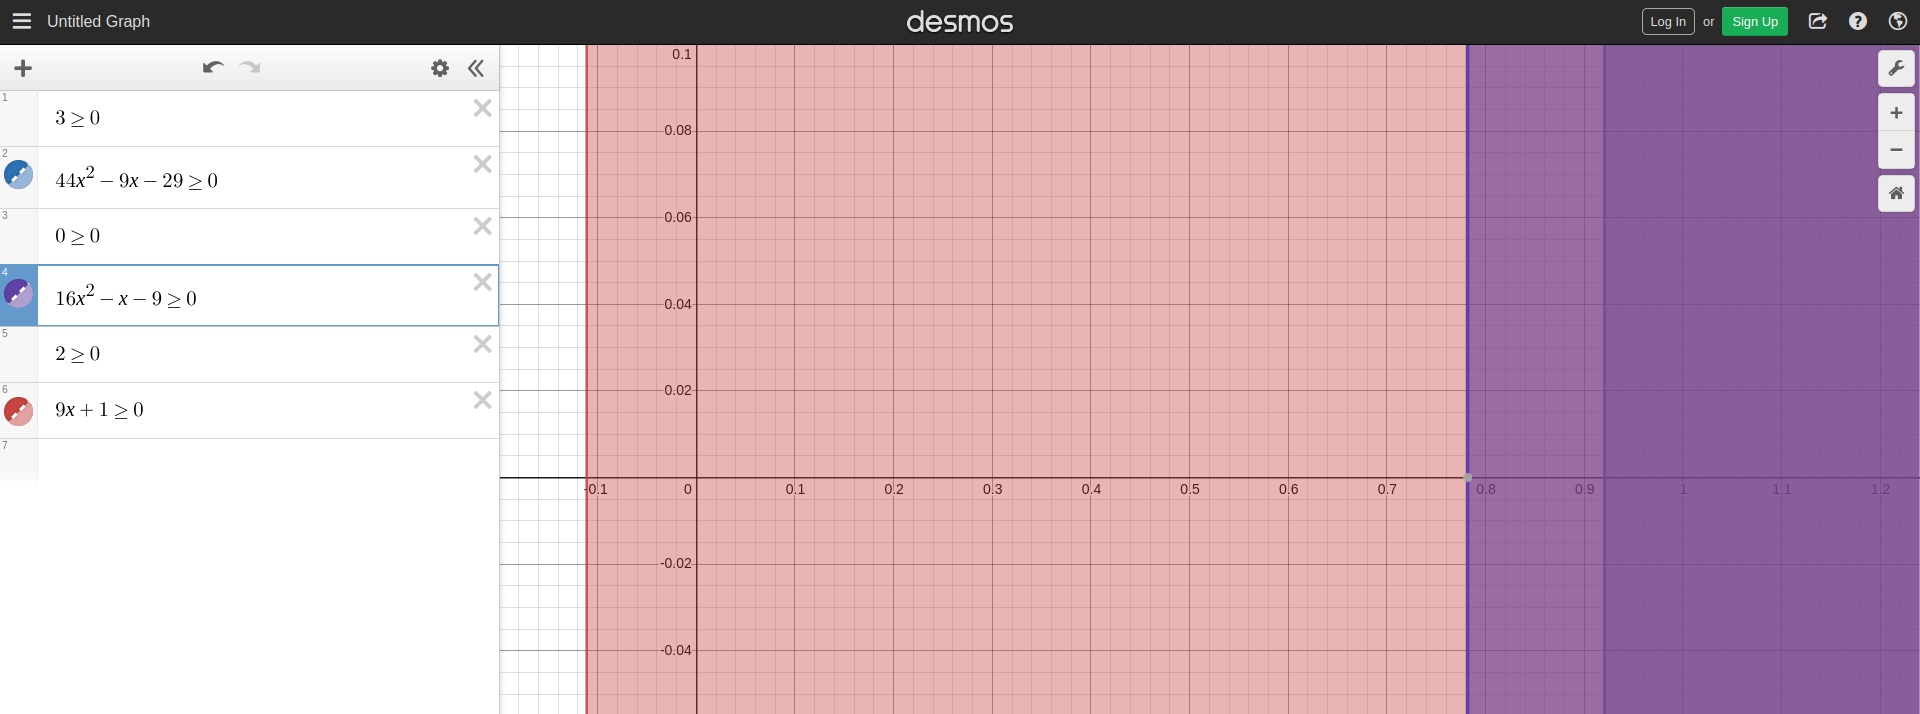
\includegraphics[scale=.3]{Phase2_iteration6_visual_updated}
\end{center}

So, by replacing $x_{11}$ with $\lambda$ in the RHS of the tableau above, we find the $5^{\text{th}}$ invariancy region that was not found using the mpLCP MATLAB implementation.

$x_{[1]}^2
 + 1$

\end{document}
